\documentclass{article}

% Language setting
% Replace `english' with e.g. `spanish' to change the document language
% \usepackage[english]{babel}
\usepackage[fontset=ubuntu]{ctex}

% Set page size and margins
% Replace `letterpaper' with `a4paper' for UK/EU standard size
\usepackage[letterpaper,top=2cm,bottom=2cm,left=3cm,right=3cm,marginparwidth=1.75cm]{geometry}

% Useful packages
\usepackage{amsmath}
\usepackage{graphicx}
\usepackage[colorlinks=true, allcolors=blue]{hyperref}
\setlength{\parindent}{2em}

\title{Merlin Bridge白皮书}
\author{Eason.Z \\dev@merlinprotocol.org \and Rilke \and shier \and Hannah}
\date{DRAFT Version 0.2.0}
\begin{document}
\maketitle

\begin{center}
\Large\textbf{一场构思伟大的诡计}
\end{center}

\begin{abstract}
随着加密货币的迅猛发展,比特币和以太坊已成为行业中两个最大的生态系统。比特币作为首个区块链落地应用,被誉为"数字黄金",其安全性和价值储存特性在加密资产市场占据重要地位。以太坊则是一种多功能的区块链科技平台,为智能合约和去中心化应用(DApps)的开发提供了广泛的可能性。随着区块链技术的不断发展,比特币跨链到以太坊的需求日益增长,截至2022年3月,已有218亿美元的资产被锁定在跨链协议中,其中WBTC\cite{wbtc}占比超过50\%。然而,超过90\%的桥梁是通过中心化托管的方式实现跨链资产转移。在2023年5月,跨链协议Multichain宣布紧急停止运营,导致其系统内锁定的价值达12.6亿美元的资产无法进行转移。Merlin Bridge是一个领先的去中心化且无需信任的协议级比特币跨链解决方案。该解决方案允许任何人通过协议向用户提供跨链通道服务,赚取相应的服务费。重要的是,该协议是完全去中心化和无需信任的,用户可以在不依赖第三方的情况下进行跨链操作。在Merlin Bridge中,协议的管理方式采用了DAO(去中心化自治组织)的模式,实现更加社区化和民主化的决策机制。这意味着社区成员可以共同参与协议的管理和治理,确保协议的发展与优化符合整体利益。
\end{abstract}

\section{跨链通道可以解决这些问题}
\par “将比特币存放在一个商业托管机构,或是分散到无数个去中心化节点上,哪一种方式你觉得会更加安全?”
\par 目前,比特币托管业务在行业中占据着相当大的市场份额。许多合规机构正在为用户提供托管服务,并不断更新和升级安全技术。然而,谁也无法百分之百地保证类似“门头沟盗币”事件不会再次发生。假设一家体量庞大的托管机构出现安全问题,不仅会影响相关业务,甚至可能对整个Web3行业造成巨大冲击(可参考“门头沟”事件)。
\par 通过将用户托管的比特币分散到众多节点上,即使某些节点出现安全问题,也不会影响整个系统的资产安全,从而实现了高度容错性。基于这一理念,我们设计了跨链服务通道。这个通道与闪电网络\cite{ln}的微支付通道\cite{bitcoinjmicropay}类似,具备通道容量和资产质押等特征,同时我们也希望 Merlin Bridge能够像Lightning Network一样,积极地推动比特币生态的扩展。
\par 跨链通道的核心功能是接收用户锁定在跨链桥中的比特币,跨链通道的创建者会在以太坊网络上进行其他资产的超额质押,以确保托管比特币的安全性。当跨链通道发生恶意行为时,可以通过拍卖清算通道质押资产的方式,保障比特币资产的安全。

\section{核心问题}
\begin{itemize}
    \item 如何保证锁定在协议中的比特币安全性?
    \item Bridge-in:如何保证比特币进入以太坊网络时MBTC不会增发?
    \item Bridge-out: Wrapped Bitcoin销毁后如何保证用户提取的比特币一定会到账?
\end{itemize}

\section{背景知识}
\subsection{Merlin Bitcoin(MBTC)}
\par 比特币进入以太坊后的ERC-20标准代币,比特币1:1锚定。
\subsection{区块}
\subsubsection{比特币}
\begin{figure}[h]
\centering
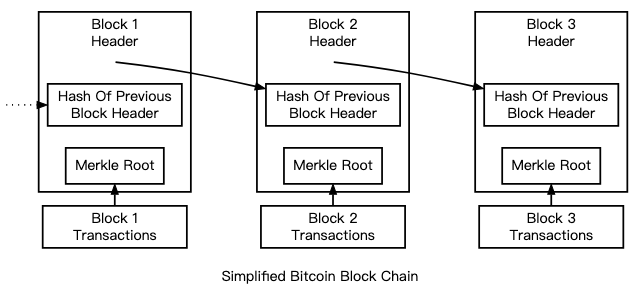
\includegraphics[width=0.85\textwidth]{bitcoin_block.png}
\caption{\label{fig:bitcoin_block}Simplified Bitcoin Block.}
\end{figure}
\par 在比特币协议中一个或多个新交易的区块被收集到区块的交易数据部分中\cite{nakamoto}。每个交易的副本都会被哈希,然后哈希被配对、哈希、再次配对、再次哈希,直到剩下一个哈希,即MerkleTree的根。Merkle根存储在区块头中。每个块还存储前一个块头的哈希值,将块链接在一起。这确保了在不修改记录该事务的块以及所有后续块的情况下无法修改该事务。
\subsubsection{以太坊}
\begin{figure}[h]
\centering
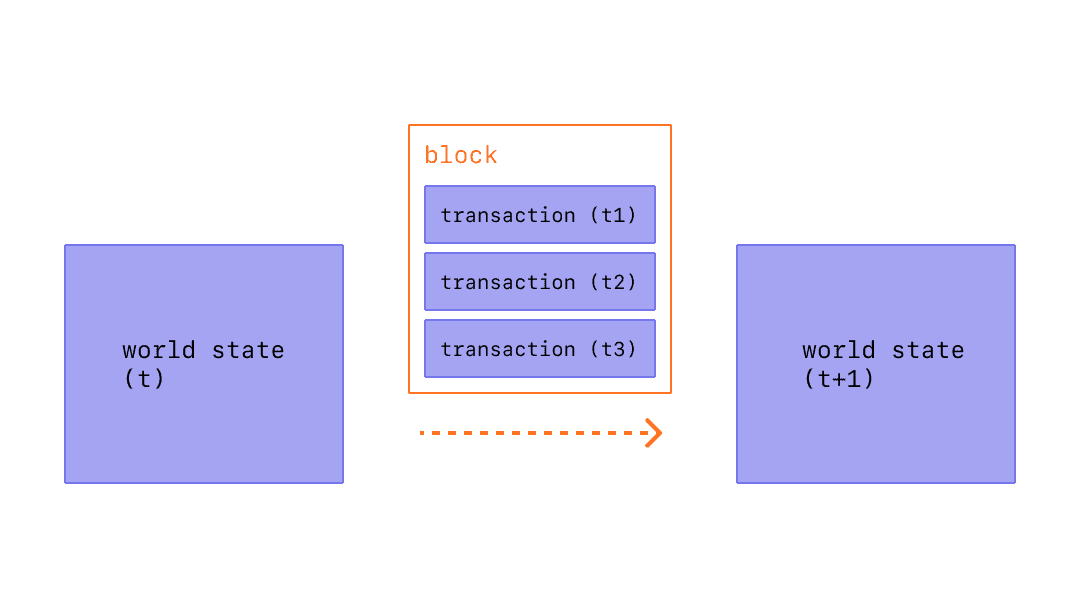
\includegraphics[width=0.85\textwidth]{eth_block.png}
\caption{\label{fig:eth_block}Simplified Ethereum Block.}
\end{figure}
\par 为了保留交易历史记录,块是严格排序的(创建的每个新块都包含对其父块的引用),并且块内的交易也是严格排序的。除了极少数情况外,在任何给定时间,网络上的所有参与者都就区块的确切数量和历史达成一致,并正在努力将当前实时交易请求批量处理到下一个区块中。一旦网络上随机选择的验证器将一个块组合在一起,它就会传播到网络的其余部分;所有节点都将此块添加到其区块链的末尾,并选择一个新的验证器来创建下一个块。\cite{ethpaper}
\subsection{UTXO与账户模型}
\subsubsection{Unspent Transaction Output (UTXO)}
\par 比特币采用UTXO模型来管理账户余额和交易输出,每笔交易至少有一个输入和一个输出。每个输入都会花费支付给前一个输出的聪。然后,每个输出都会作为未花费的交易输出(UTXO)等待,直到稍后的输入将其花费。当您的比特币钱包告诉您有 10,000 聪余额时,这实际上意味着您有 10,000 聪在一个或多个 UTXO 中等待。
\begin{figure}[h]
\centering
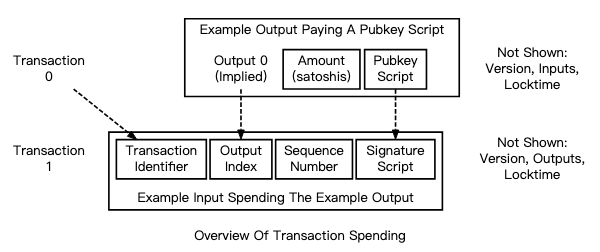
\includegraphics[width=0.85\textwidth]{utxo.png}
\caption{\label{fig:utxo}Overview of Transaction Spending.}
\end{figure}
\par 当一笔比特币交易被确认后,其输入将被标记为已使用,而输出则会成为新的未使用交易输出,等待被后续的交易消费。
\subsubsection{账户模型}
\begin{figure}[h]
\centering
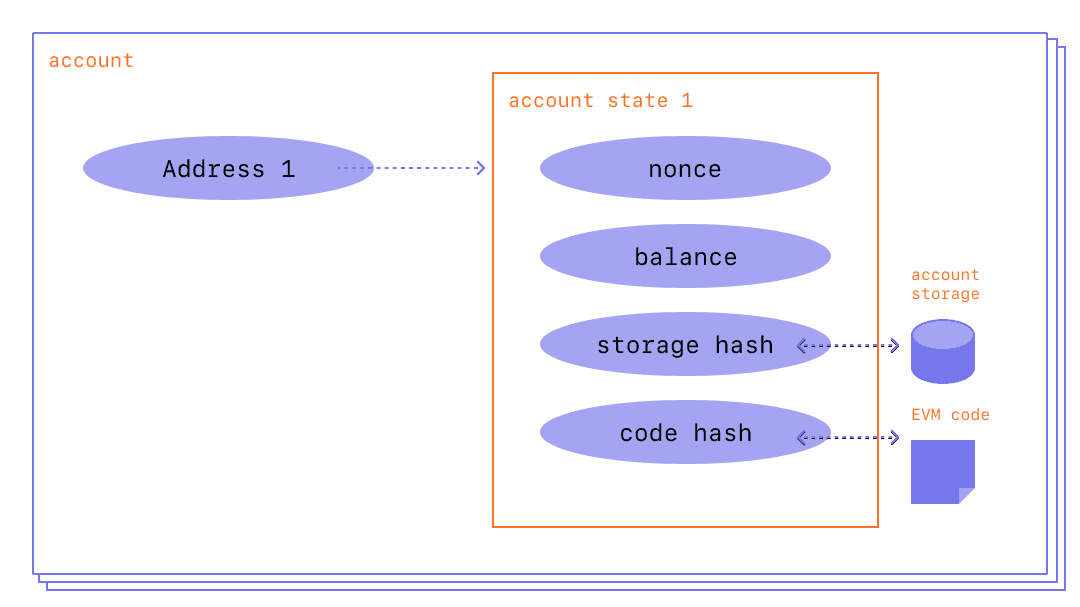
\includegraphics[width=0.85\textwidth]{account.png}
\caption{\label{fig:account}Overview of Ethereum Account.}
\end{figure}
\par 以太坊账户是一个具有以太坊 (ETH) 余额的实体,可以在以太坊上发送交易。帐户可以由用户控制或部署为智能合约。\\
帐户的作用:
\begin{itemize}
    \item 接收、持有和发送ETH和代币
    \item 与已部署的智能合约交互
\end{itemize}
以太坊账户有四个字段:
\begin{itemize}
    \item nonce– 一个计数器,指示从外部拥有的账户发送的交易数量或合约账户创建的合约数量。每个账户只能执行一笔具有给定随机数的交易,从而防止签名交易被重复广播和重新执行的重放攻击。
    \item balance– 该地址拥有的wei数量。Wei是ETH的面额,每个ETH有1e+18wei。
    \item codeHash– 该哈希值指的是以太坊虚拟机(EVM)上的帐户代码。合约账户中编写有可以执行不同操作的代码片段。如果帐户收到消息调用,则会执行此EVM代码。与其他帐户字段不同,它无法更改。所有此类代码片段都包含在状态数据库中相应的哈希值下,以供以后检索。该哈希值称为codeHash。对于外部拥有的帐户,codeHash 字段是空字符串的哈希值。
    \item storageRoot– 有时称为存储哈希。Merkle Patricia trie根节点的256位哈希,对账户的存储内容(256 位整数值之间的映射)进行编码,作为来自256位的Keccak256位哈希的映射编码到trie中。RLP编码的256位整数值的位整数密钥。这个trie编码了这个账户的存储内容的hash,默认为空。
\end{itemize}

\subsection{智能合约与比特币签名脚本}
\subsubsection{比特币签名脚本}
\par 比特币签名脚本是一种基于堆栈的简单脚本语言,用于验证比特币交易中的输入和输出。它被用于确保只有合法的交易能够被添加到区块链中,从而维护比特币的安全性和完整性。比特币签名脚本由一系列操作码(OP\_Code)和数据项组成,以字节码的形式存在。在交易中,输入脚本和输出脚本分别附加在输入和输出上,用于验证交易的合法性。\cite{wikicontracts}\\
以下是几种常见的签名脚本类型:
\begin{itemize}
    \item Pay-to-Public-Key-Hash (P2PKH): P2PKH是最常见的比特币签名脚本类型。在P2PKH交易中,输出脚本包含接收者的公钥哈希。为了解锁这笔交易输出,发送者必须提供与公钥相对应的签名和原始公钥。这种签名脚本通常以“OP\_DUP OP\_HASH160 <PubKeyHash> OP\_EQUALVERIFY OP\_CHECKSIG”形式表示。
    \item Pay-to-Script-Hash (P2SH): P2SH是一种用于多重签名和更复杂脚本的签名脚本类型。在P2SH交易中,输出脚本包含一个脚本哈希,该脚本哈希对应于接收者的脚本。发送者必须提供与接收者脚本相匹配的解锁脚本,以解锁输出。这种签名脚本通常以“OP\_HASH160 <ScriptHash> OP\_EQUAL”形式表示。
    \item Pay-to-Witness-Public-Key-Hash (P2WPKH): P2WPKH是隔离见证(Segregated Witness,简称SegWit)的一种形式。在P2WPKH交易中,输出脚本包含接收者的公钥哈希,而解锁脚本直接包含与公钥相对应的签名。这种签名脚本通常以“<Signature> <PublicKey>”形式表示。
    \item Pay-to-Witness-Script-Hash (P2WSH): P2WSH也是SegWit的一种形式,用于支持多重签名和其他复杂脚本。在P2WSH交易中,输出脚本包含一个脚本哈希,而解锁脚本包含与接收者脚本相匹配的数据。这种签名脚本通常以“0 <ScriptHash>”形式表示。
\end{itemize}
\subsubsection{智能合约}
\par “智能合约”只是在以太坊区块链上运行的程序。它是驻留在以太坊区块链上特定地址的代码(其功能)和数据(其状态)的集合。
\par 智能合约是以太坊账户的一种。这意味着他们有余额并且可以成为交易的目标。然而,它们不受用户控制,而是部署到网络并按编程运行。然后,用户帐户可以通过提交执行智能合约上定义的功能的交易来与智能合约进行交互。智能合约可以像常规合约一样定义规则,并通过代码自动执行它们。智能合约默认无法删除,并且与智能合约的交互是不可逆的。
\subsection{预言机}
\par 在智能合约中,预言机是一种机制,用于将外部数据引入到区块链中,使智能合约能够与现实世界的信息进行交互。由于智能合约本身无法直接访问外部数据,预言机充当了连接区块链和现实世界的桥梁,为智能合约提供了外部数据的输入\cite{oralce}。
在智能合约中,预言机可以用于许多用途,例如:
\begin{itemize}
    \item 提供价格数据:智能合约可以使用预言机来获取现实世界的价格数据,用于执行条件和触发合约操作,如期权合约、保险合约等。
    \item 外部事件触发:预言机可以用于将外部事件(如天气、体育比赛结果等)引入智能合约,并触发相应的合约逻辑。
    \item 跨链交互:在跨链交互中,预言机可以用于获取其他区块链网络上的数据,实现区块链之间的互操作性。
\end{itemize}
\subsection{SPV(Simplified Payment Verification)}
\par 在比特币协议中不运行一个完整的网络节点也是可以进行支付验证的。用户只需拥有一个最长工作量证明链的区块头副本,他可以通过向其他网络节点查询以确认他拥有了最长的链,并获取链接交易到给交易打时间戳区块的Merkle分支。虽然他自己不能核实这个交易,但如果交易已经链接到链中的某个位置,就说明一个网络节点已经接受了此交易,而其后追加的区块进一步确认网络已经接受了它。\cite{spv}
\begin{figure}[h]
\centering
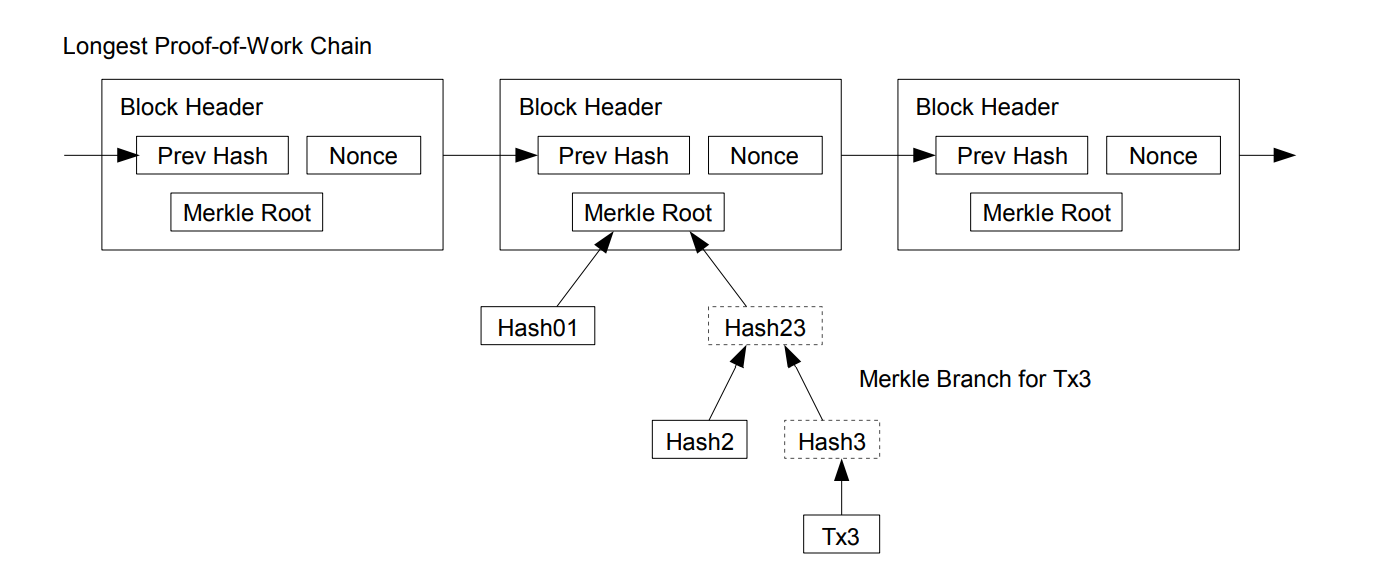
\includegraphics[width=0.85\textwidth]{spv.png}
\caption{\label{fig:spv}Overview of Simplified Payment Verification.}
\end{figure}
\par 只要诚实节点依然在掌控网络,如此这般,验证即为可靠的。然而,如果网络被攻击者所控制的时候,验证就没那么可靠了。尽管网络节点可以自己验证交易记录,但是,只要攻击者能够继续控制网络的话,那么简化版验证方式可能会被攻击者伪造的交易记录所欺骗。应对策略之一是,客户端软件要接受来自网络节点的警告。当网络节点发现无效区块的时候,即发出警报,在用户的软件上弹出通知,告知用户下载完整区块,警告用户确认交易一致性。那些有高频收付发生的商家应该仍然希望运行属于自己的完整节点,以此保证更独立的安全性和更快的交易确认。
\subsection{跨链原子级互换}
\par 原子交换使用哈希时间锁定合约(HTLC)(一种脚本合约)来促进资产的去信任交换\cite{lamportclocks}。脚本合约采用自动化流程,一旦满足合约中编码的所有预定条件,该流程就会自动执行。\\
比特币原子交换的实现得益于比特币 HTLC 中编码的两个关键组件:
\begin{itemize}
    \item 哈希锁:哈希锁是由发起交易的人生成的加密隐藏密钥。该密钥确保只有在双方都批准交易后,交换才会最终完成。
    \item 时间锁:时间锁是作为检查锁定时间验证命令 (CLTV) 或检查序列验证 (CSV) 创建的。使用 CLTV,交易中的资金根据日期和时间被锁定或释放。使用 CSV,资金在生成一定数量的区块后被锁定或释放。简而言之,时间锁设定了交换的最后期限。如果双方在规定时间之前未批准交换,则时间锁将充当安全机制并使交易无效。在这种情况下,资金将被送回各自的所有者。
\end{itemize}
\section{架构}
\subsection{角色与职责}
\subsubsection{开发者社区}
\par 开发者社区是Merlin Protocol生态系统的重要组成部分,他们承担着项目的开发与创新工作。在早期阶段,由Merlin基金会主导并提供资金支持。开发者社区致力于构建一系列服务于Bridge的区块链基础设施智能合约。他们的工作将确保Merlin Protocol的顺利运行和持续发展。\\
负责系统:
\begin{itemize}
    \item 链上数据监控系统,负责监控跨链服务提供商交易行为;
    \item 链下智能合约触发器;
    \item 清算系统;
\end{itemize}
\subsubsection{跨链通道服务提供商}
\par Merlin Bridge欢迎任何人成为跨链通道服务提供商,为Merlin Bridge的顺利运行贡献力量。对应跨链通道服务提供商可以赚取到1.5\%的交易手续费(后续会有社区投票治理设定)。
\begin{figure}[h]
\centering
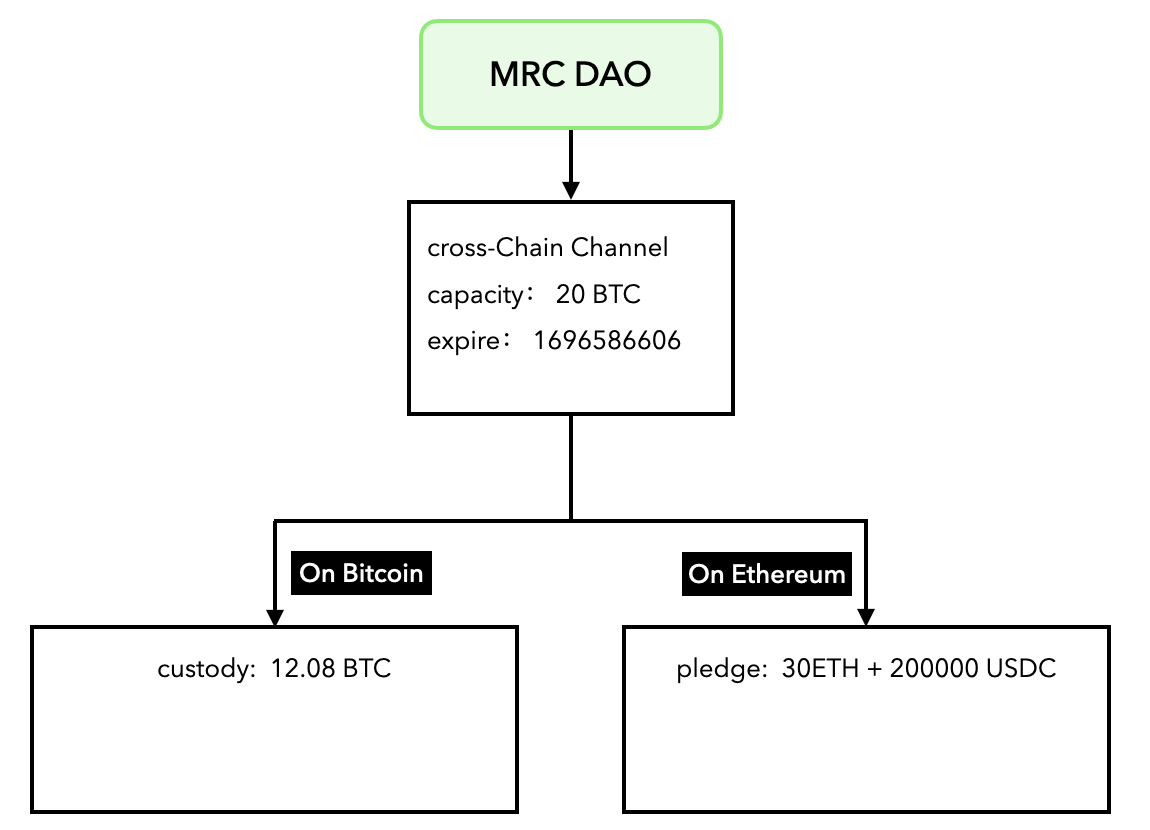
\includegraphics[width=0.85\textwidth]{services.png}
\caption{\label{fig:services}Accounts with Cross-chain Channel.}
\end{figure}
\par 跨链通道涵盖两个账户:一个位于比特币网络,另一个为以太坊账户。比特币公钥用于接收用户在通道中托管的资产,而通道服务提供商将通过在以太坊账户中超额质押链上资产,以维持通道容量。这种超额质押的资金有效地保障了比特币资产的安全。\\
流程:
\begin{itemize}
    \item 向开发者社区提交申请,并提交用于比特币锁定的公钥(为了减轻预言机的负担,协议要求提的托管地址并未在比特币网络中出现过)。经过开发者社区的审核后,将注册到预言机合约中提供比特币网络查询服务;
    \item 生成比特币接收地址后,该地址将被添加到预言机SPV服务中,成为智能合约编程的数据源;
    \item Merlin Bridge网关显示;
\end{itemize}
\subsubsection{预言机集群}
\par 预言机集群是一个以太坊智能合约和链下服务器集群组成的系统,用于将比特币网络中特定地址的交易数据上链。其主要作用是通知智能合约有关比特币网络中监控地址余额变化的信息。通过预言机集群,智能合约可以实时获得比特币网络的数据更新,进而执行相应的逻辑和操作。
\subsubsection{清算者}
\par 清算者是指参与Merlin Bridge清算拍卖的用户。他们可以通过使用比特币来购买处于不稳定状态的债务,获得抵押资产并参与拍卖过程。清算者的参与对于维持MBTC的稳定性非常重要,因为他们通过拍卖机制确保跨链通道服务提供商质押物的清算,从而避免通道服务商作恶的风险。
\subsubsection{用户}
将比特币转换成MBTC,使其在以太坊智能合约中可用,并参与各种以太坊生态系统的活动。
\subsection{跨链过程}
\subsubsection{模块介绍}
跨链通道:
\par 跨链服务节点是运行在服务器上的可执行程序,负责处理业务逻辑、智能合约交互以及与web3钱包的交互。\\
节点的主要属性:
\begin{itemize}
    \item 通道状态:未激活、激活、冻结、暂停、关闭。
    \item 通道容量:每个节点都具有预先确定的跨链通道容量,即它可以托管的比特币数量上限。这个通道容量在节点激活之前就已经确定,确保节点在运行期间始终拥有稳定的跨链资产处理能力。
    \item 通道最小容量:与微型支付相似通道设有最小容量限制,用以保证跨链服务质量与稳定性。
\end{itemize}
通道网关:
\par Merlin Bridge由无数个跨链通道组成,用户在进行跨链操作之前需要通过网络选择符合条件的通道进行操作。通道排序支持容量上限、可用金额和跨链资产总量排序,方便用户根据自身需求进行选择。\\
公共通道:
\par 在生态早期发展阶段,为确保通道平稳运行,为用户提供优质跨链服务,基金将负责构建和维护公共跨链通道。当其他通道发生异常导致比特币需要清算时,这些比特币将被托管至公共通道。预计在未来两年内,随着通道数量规模的增长,基金会将逐步关闭公共通道。
\subsubsection{实现比特币网络到以太坊网络的代币跨链转移}
\par 跨链转移的难点在于确保两条链上交易状态的一致性,其中包括交易顺序、代币数量以及在失败情况下的交易回滚。\\
最简化的流程:
\begin{enumerate}
    \item 用户可通过在比特币网络上发起一笔交易,将比特币转入跨链通道
    \item 跨链通道实现比特币交易数据同步,将对应账户的比特币转移为MBTC
\end{enumerate}
\par 最简单的方法是将完整的比特币交易数据存储在智能合约中,但显然这样做并不现实。不过,可以将相关的交易数据存储在以太坊智能合约之外,并通过预言机来查询所需的交易数据。理论上,这样可以在智能合约内部验证比特币交易的有效性,从而确保在比特币进入以太坊网络时不会增发MBTC。
\par 在此,我们采用SPV(Simplified Payment Verification)来验证比特币交易的有效性,数据源由预言机提供,并在智能合约中实现验证算法。
\begin{figure}[h]
\centering
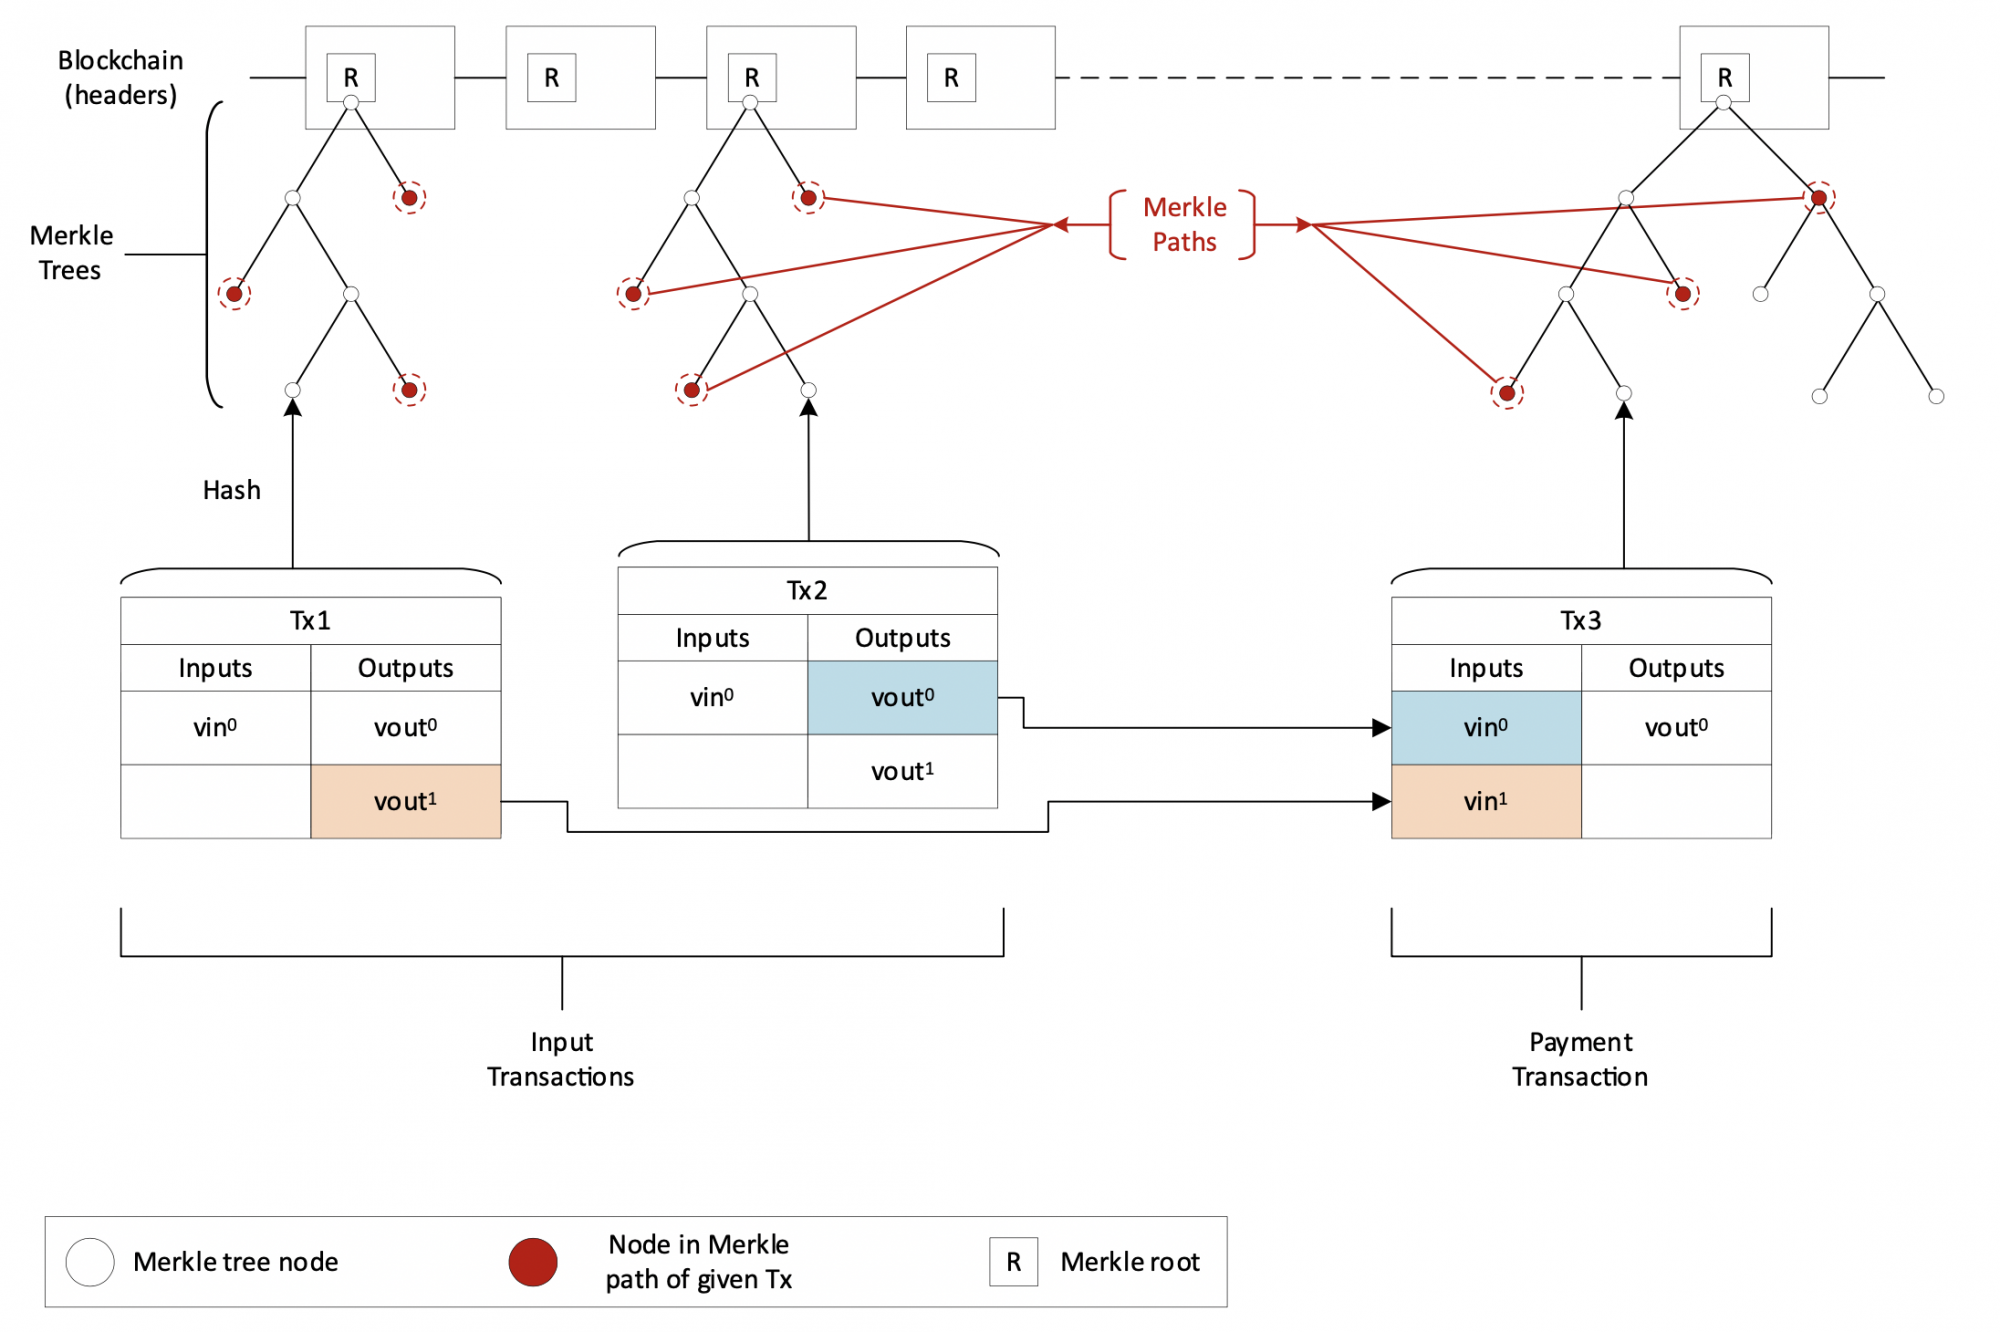
\includegraphics[width=0.85\textwidth]{spv2.png}
\caption{\label{fig:spv2}Verification.}
\end{figure}
\par 比特币的交易由input和output组成,其中input本质上是之前发生的某一笔交易的output。为了验证交易的存在性,需要进行1+n次Merkle运算:
\begin{enumerate}
    \item Bridge-in交易哈希的Merkle路径,并在预言机中查询区块头是否存在
    \item Bridge-in交易中n个Input的Merkle路径,并在预言机中查询区块头是否存在
\end{enumerate}
\par 交易对应的Merkle路径由业务系统提供,以数组的方式传入智能合约执行。在Solidity中,Merkle计算已得到支持,并广泛应用于多个领域,例如NFT的白名单设置中。接下来要解决预言机数据存储的问题。
\par 预言机向合约提供SPV查询服务需要存储所有的比特币区哈希,其中比特币区块头的大小为80个字节,目前所有头部约占用60M的存储空间。考虑到预言机的负担,协议将选择一个指定高度进行SPV查询服务提供,预计是第750000高度,在此之前的MerkleRoot哈希将无法在预言机中查询到。在跨链通道中,我们会采取一些业务保护措施,要求用户先进行一次归整交易,确保输入交易发生在服务高度之后,然后再进入跨链通道。虽然这可能造成一些不便,但对于系统的稳定性将大幅提升。
\par 智能合约已经可以通过预言机确定一笔交易是否在比特币网络上存在。接下来的关键问题是解决交易细节的解析,主要包括验证输出脚本是否符合协议标准。
% \par 比特币交易的平均大小约为250个字节。交易的大小与转账数量无关,而是与input和output的数量有关。当input和output的数量增加时,会导致比特币交易的膨胀。为了减少智能合约传入的数据流,协议规定Bridge-in的交易input不能超过3个,output不超过2个。这样的限制有效控制了交易的大小,确保合约的正常运行,并保障了网络的高效性和安全性。
\subsubsection{Bridge-in tx汇集}
\par 在比特币网络中,当用户发起bridge-in交易时,很难实现对以太坊上通道容量的有效性判断。举个例子,假设一个通道的容量只剩下0.5个BTC,此时有5个用户在一个区块中向该通道发起了0.2个BTC的交易。这样的情况下,当这些交易被打包进区块后,可能会导致通道的保证金比例降低到150\%以下,这会增加通道服务商作恶的风险。
\par 解决思路是对通道的Bridge-in交易进行合并,并实现交易回滚:
\begin{figure}[h]
\centering
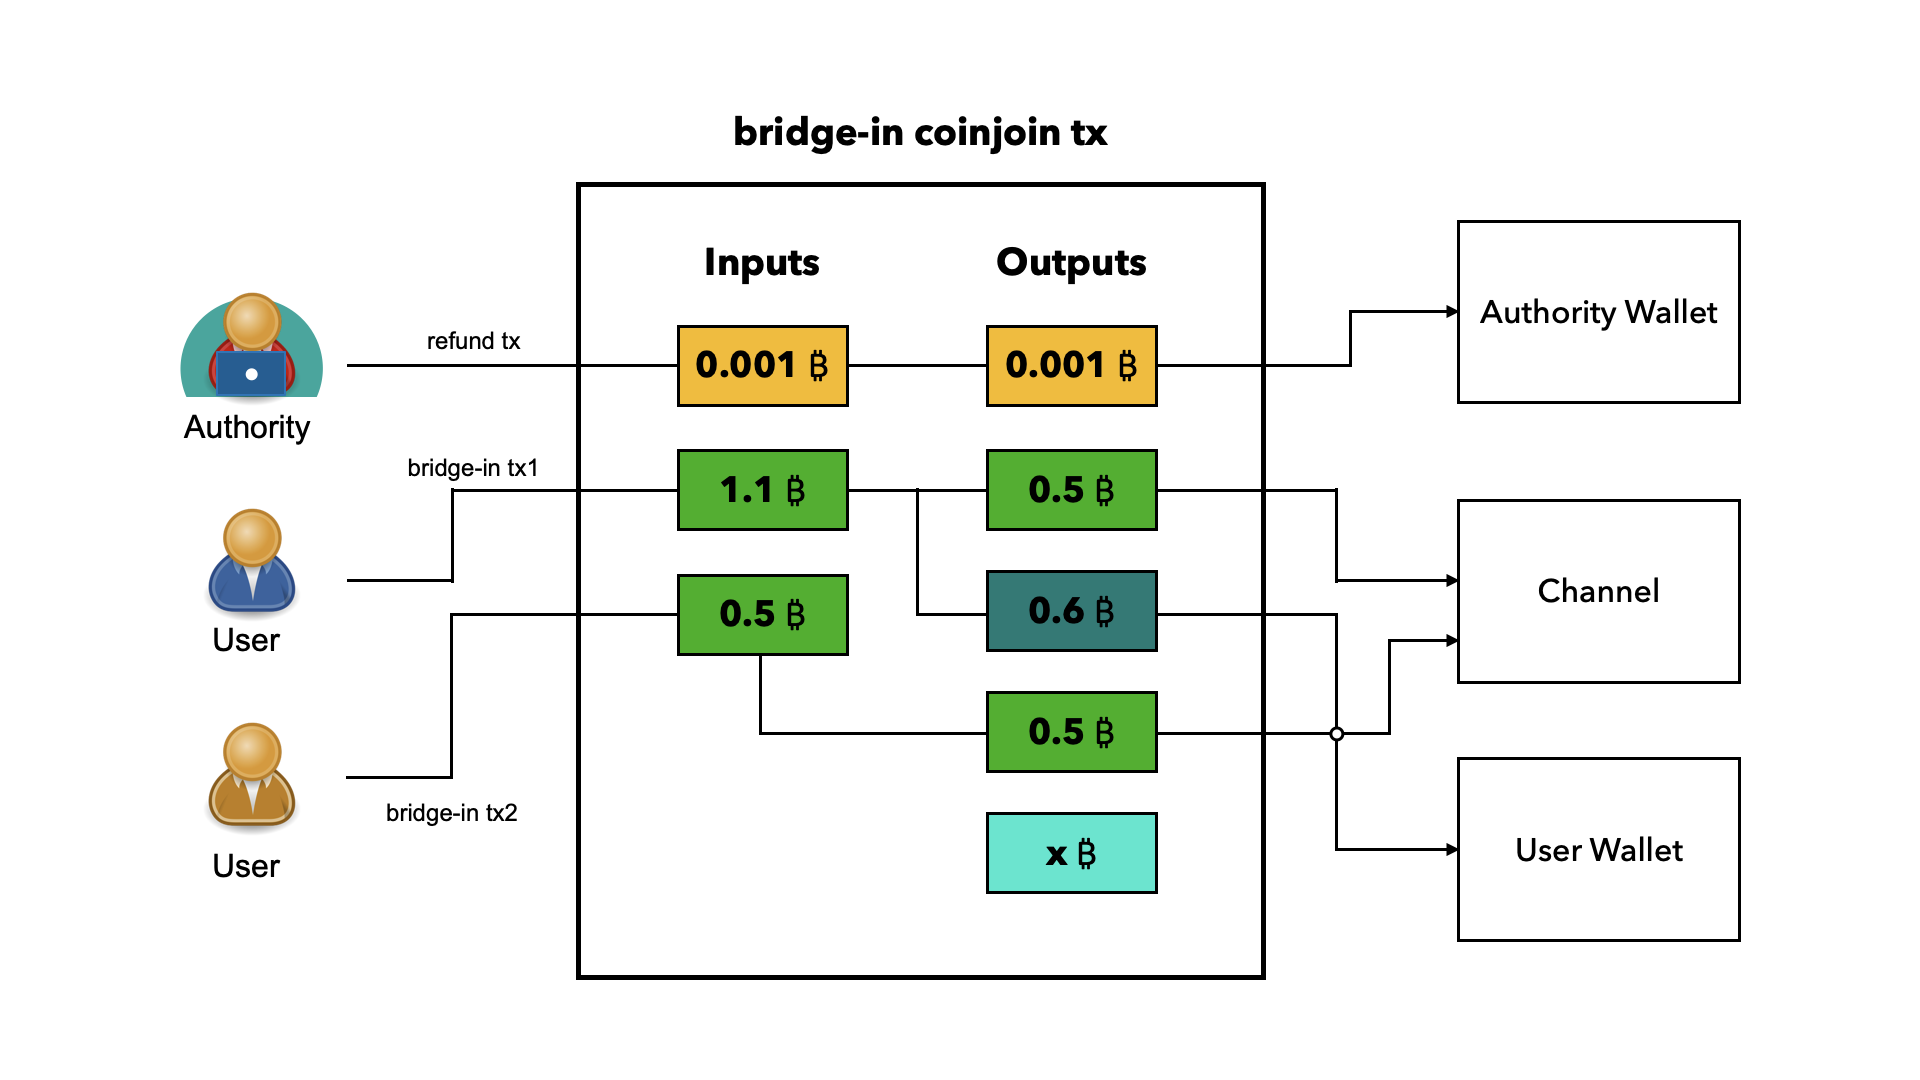
\includegraphics[width=0.85\textwidth]{coinjoin.jpg}
\caption{\label{fig:coinjoin}Bridge-in coinjoin tx.}
\end{figure}
\par 通过CoinJoin技术,对目标为相同跨链通道的Bridge-in交易进行了汇集处理。同时,引入了一笔官方发送的Refund交易,以增强交易的安全性。在汇集交易中,通过设置locktime参数,使其在交易池中等待2个区块的确认。我们的链下监控系统会持续监控比特币交易池,并进行深入分析,以确保进入通道的比特币不会导致保证金比例失衡。一旦监控系统检测到异常情况,它将发起一笔refund交易,在汇集交易执行之前消耗掉一个input,从而使汇集交易无效。这种设计的安全机制保障了用户资金的安全,并确保交易的可靠性和稳定性。
\par 基于这种设计实现了三个功能:
\begin{itemize}
    \item 对Refund进行染色处理,更好的捕获Bridge-in交易类型
    \item 实现了通道交易的一致性以及交易撤销
    \item 可以通过Refund交易向用户补贴发生在比特币网络的手续费
\end{itemize}
\subsubsection{交易染色}
\par 为了与其他交易区分开来,我们设计了一套简单而实用的协议标准,将其嵌入到输出脚本中,以实现Bridge交易的标识。通过在比特币交易中对输出脚本进行染色,以便能够清晰地区分Bridge交易与其他交易类型。
\begin{figure}[h]
\centering
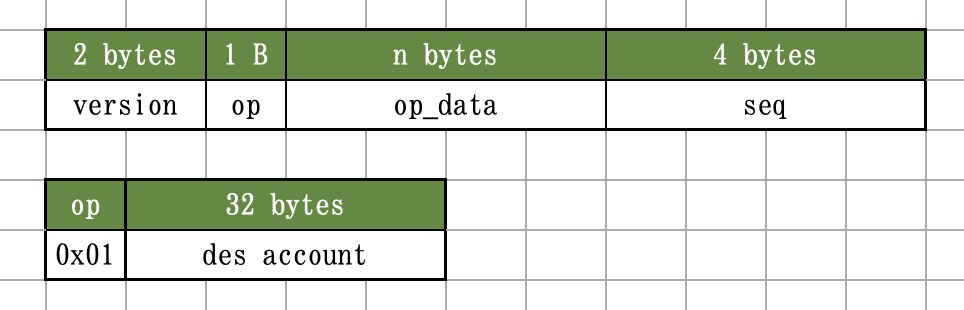
\includegraphics[width=0.85\textwidth]{bytes.jpg}
\caption{\label{fig:bytes}Protocol Format.}
\end{figure}
\begin{enumerate}
    \item 2个字节长度表示协议版本号,版本号从0x0001开始累加,每个版本号对应不同的解析规范,实现协议升级兼容
    \item 1个字节表示operator code,根据op类型进行后续字节的解析
    \item op\_data为具体操作数据长度不确定
    \item 4个字节用以表示序列号(sequence number)
\end{enumerate}
\par 当op为0x01时表明交易为bridge-in交易,具体op\_data解析规则如下:
\begin{itemize}
    \item 32个字节目标账户地址
\end{itemize}
\par 为了减少比特币交易的大小,会将协议的二级制数据进行hash256得到32个字节的唯一标识再附加在output脚本中
\begin{verbatim}
OP_FALSE
OP_IF
  OP_PUSH 0x00000...
  OP_PUSH 1
OP_ENDIF
\end{verbatim}
\par 脚本中的OP\_FALSE OP\_IF … OP\_ENDIF用于包装一定数量的数据。需要注意的是,这些脚本实际上是无操作的,它们不会改变包含它们的脚本的语义。最终,这些脚本将附加在花费比特币UTXO(未使用交易输出)的具体内容上。
\par MBTC的国库智能合约将负责处理以太坊链上的MBTC增发和销毁功能,其流程如下:
\begin{enumerate}
    \item 用户发起一笔bridge-in交易,并将其写入区块链中。
    \item 预言机更新区块头部数据,以确保MBTC的状态与比特币网络同步。
    \item 合约调用MBTC国库的Mint方法,向用户铸造相应数量的MBTC代币。
    \begin{enumerate}
        \item 交易有效性验证
        \item 跨链通道以及容量有效性验证
        \item Bridge-in交易标识
        \item 增发MBTC
    \end{enumerate}
\end{enumerate}
\par 合约允许任意以太坊账户调用触发MBTC铸造功能,而不设权限限制。现在我们已经实现了比特币在以太坊网络上的1:1增发。

\subsubsection{以太坊网络MBTC的销毁与比特币主网赎回}
\par 跨链通道服务提供商拥有用户托管比特币的控制权,因此存在着潜在的作恶动机。为确保跨链通道的正常运行和用户资产的安全,我们采用了类似FileCoin超额质押与作恶罚没的方式约束通道行为规范。
\begin{itemize}
    \item 跨链通道需要质押价值其通道150\%的资产作为保证金;
    \item 当用户在通道Bridge-out比特币时将获得1.5\%的手续费;
\end{itemize}
流程:
\begin{enumerate}
    \item 用户通过MBTC国库合约发起比特币赎回事务,合约将销毁相应的MBTC,并记录比特币接收地址以及所使用的通道信息;
    \item 跨链通道即时捕获合约发起的事务,解析其中的数据,然后向用户发起相应数量的比特币转账;
    \item 预言机将捕获这笔比特币交易,并将其数据上链;
    \item 跨链通道服务顺利完成事务,并将其关闭;
\end{enumerate}
\subsubsection{MBTC的质押与清算}
\par 由预言机喂价,提供不同资产的价格,包括BTC、ETH以及实际参与抵押的链上资产。不同通道计算已铸造的MBTC价值与总共抵押资产的价值。这一环节不需要链上实时计算,提供前端页面即可。
\par 实时计算各个通道承担的MBTC的负债与抵押物的抵押率。当资产总抵押率低于120\%时,清算者可清算该节点的部分资产以维持抵押率。当抵押率低于110\%时,基金会将清算全部抵押资产。
\par 清算者(其他通道节点,白名单清算者,基金会成员)可以发起部分清算交易。向公共通道支付任意数额的BTC后,向合约申请清算任意节点的抵押资产。 合约会尝试等比例扣除总价值为支付BTC105\%的抵押资产,并支付给清算发起方。 但是部分清算交易生效的条件是计算清算掉BTC和对应价值的抵押物之后,资产总抵押率低于120\%\cite{aavev3}。 
测算:
\begin{itemize}
    \item 假设当前抵押率下跌至116\%,以总价值\$400的MBTC和\$465的抵押资产组合为例。则最多可能被清算的资产为25\%的资产,即清算\$100的MBTC和\$105的抵押资产组合,剩余资产为总价值\$300的MBTC和\$360的抵押资产组合,抵押率即可恢复至120\%,节点承担的损失仅为\$5,相对总抵押资产仅约为1.1\%的比例,风险敞口较低。
    \item 清算后,该节点承兑BTC的义务额度减少\$100,且公共通道的承兑义务增加100\$。后续BTC承兑优先由公共通道完成。
    \item 清算者进行清算时,也可以自行发行MBTC,使用自由的MBTC支付给欠抵押节点,进行清算交易。 被清算节点将强制支付相应数量的抵押资产组合换取MBTC。当节点履行承兑义务时,可以启用持有的其他节点MBTC进行承兑。
\end{itemize}
\par 初始抵押率为150\%,这既可以保持资产在一定下跌幅度时不会马上达到清算线,也保证了较高的资金利用率和资产收益率,维持安全与收益的平衡
\par 根据近年来数据,BTC和ETH收益率相关系数为87\%,极高的资产相关性将保证在大幅行情变动中抵押率的稳定。 而ETH的收益率波动为BTC的1.25倍(该数字实际值为1.1),结合初始150\%的抵押率和65\%ETH+35\%USD的资产组合,可以得到总抵押资产组合对比特币的币价波动比例为1.5*65\%*1.25=1.22。这一资产组合设置可以天然维持抵押率不会低于120\%。\\
假设节点发行了总价值\$100的MBTC,则需要\$97.5的ETH+\$52.5的USDC作为抵押资产组合:
\begin{enumerate}
    \item 在BTC价格小幅上涨情况下,假设上涨幅度为40\%,发行的MBTC总价为\$140。按照历史数据,ETH上涨的期望为50\%,则抵押资产组合的总价值为\$97.5*1.5+52.5=196.25,总抵押率为140\%,抵押率足够安全。
    \item 在BTC价格极大幅上涨情况下,假设上涨幅度为200\%,发行的MBTC总价为\$300,ETH上涨的期望为250\%,则抵押资产组合的总价值为\$97.5*3.5+52.5=388.75,抵押率为130\%仍然在安全边际内。
    \item 无论BTC涨幅多大,这一资产组合的设置可以保证从期望上抵押率不会低于1.22
    \item 在BTC价格小幅下跌情况下,假设上涨幅度为40\%,发行的MBTC总价为\$60。按照历史数据,ETH下跌的期望为50\%,则抵押资产组合的总价值为\$97.5*0.5+52.5=100,总抵押率为166\%,资产下跌将使得总抵押率更加高。
\end{enumerate}
\subsection{幽灵比特币}
\par 幽灵比特币是跨链服务通道提供的一种特殊交易,这些交易不需要真实的比特币即可增发MBTC。幽灵比特币交易要求在一个区块中完成MBTC的增发与销毁,并支付相应的交易费用。
\par 当以太坊上MBTC交易存在套利空间时,用户可以通过幽灵比特币快速进行流动性套利,且无需本金要求。幽灵比特币是MBTC独有的技术特性,基于幽灵比特币,MBTC将获得更加丰富的市场流动性。
\section{激励}
Merlin Protocol,作为一个开放生态协议,早期发展阶段将借助 MRC 代币激励生态中的有意义行为,从而推动生态系统的蓬勃发展。\\
% \subsection{MRC基础信息}
% \begin{itemize}
%     \item 总量上限:1000,000,000(10亿枚)
%     % \item 初始价格区间:0.05 USDT
%     \item 开发者团队占比:20\%(Merlin Protocol开发者团队)
%     \item 投资人占比:15\%(Merlin Protocol早期投资人分配)
%     \item 基金会:65\%(Merlin Protocol协议安全、用户增长、投资孵化、新业务扩展)
% \end{itemize}
\subsection{Token权益}
\begin{enumerate}
    \item 投票权:Merlin Protocol是一个去中心化的链上协议,在有关协议的升级和核心参数的调整过程中,需要MRC持有人作为协议的共同构建者,参与协议的公共治理。
    \item 收益权:MRC持有人可以通过 staking 的方式将MRC质押到协议中,捕获协议在参与RWA资产投资的结果收益,收益包括:MRC和加密稳定币。
    \item 使用权:MRC作为一种具备内在价值支持的加密资产,其具备一定的使用权。
    \begin{enumerate}
        \item 成为跨链通道服务商的过程中可以选择抵押一定比例的Token作为保证金;
        \item 用作RWAs相关投资
    \end{enumerate}
\end{enumerate}
\subsection{Merlin Protocol治理}
Merlin Protocol是一个去中心化的链上协议,在有关协议的升级和核心参数的调整过程中,需要MRC持有人作为协议的共同构建者,参与协议的公共治理。\\
1 MRC Token =  1 Vote \\
投票治理有2种类型:\\
\begin{enumerate}
    \item 常规投票:持有 100 万枚MRC的钱包地址,在每一次常规升级中,有7天的投票期,50\%以上赞同票视为投票通过。
    \item 紧急投票:Merlin Protocol基金会或开发者团队钱包地址在遇到紧急问题需要投票升级时,只需要流通量30\%MRC支持通过即可执行。
\end{enumerate}
\section{Merlin Bridge的前景与影响}
\par 在生态早期,通道的质押资产主要由ETH、USDT和USDC等稳定币组成。随着发展阶段的提升,我们将开放社区提案,以丰富质押资产列表。这种方式有助于使协议生成的MBTC更好地在其他生态系统中流通,从而促进双向发展。同时,随着Merlin Bridge锁定的比特币数量逐渐增加,生态治理代表MRC也将拥有更多的流动性。在符合客观条件的情况下,我们将发起社区投票,将MRC纳入通道质押资产的范围之中。
\subsection{对未来发展的展望}
以太坊生态已经全面进入Layer2时代。未来将涌现更多Layer2公链,这些公链都需要优质的资产来支撑其生态系统,创造出巨大的市场机会。在完成 Merlin Bridge以太坊跨链功能后,我们将着手支持 Layer2网络,用户可以通过我们的协议轻松进出Layer2网络,参与更多金融活动。这标志着我们在 Layer2领域的扩展,为用户带来更多机遇。

\bibliographystyle{plain}
\bibliography{references}

\end{document}